\documentclass{newsletter}

\kdrtitle{říjen 2024}
\kdrsubtitle{Newsletter komise rozhodčích a delegátů}
\kdrbackground{rijen-2024-background.jpg}

\begin{document}

\clanek{Vážení rozhodčí a delegáti,}{}
Dovolte mi vás přivítat u říjnového newsletteru od KRD USaLB. Zářijový newsletter se setkal s pozitivním ohlasem, za což jsme rádi, ale i s konstruktivní zpětnou vazbou. Nejvýraznější změnou je design, který je nyní blíže identitě Českého florbalu. Věříme, že tímto krokem dojde ke zkvalitnění newsletteru a jednodušší vizuální komunikaci informací.

Tento měsíc jsme si pro Vás připravili newsletter s následujícími tématy:
\begin{itemize}
	\item Pravidlo tří metrů a nedovolená vzdálenost
	\item Vyplácení cestovních náhrad v regionu USaLB
	\item Potvrzování zápisů a omlouvání z nominací
	\item Novinky a semináře v Listopadu
\end{itemize}

KRD bude opět ráda za jakoukoliv zpětnou vazbu, která nám pomůže vylepšit newslettery do budoucna tak, aby Vám co nejlépe pomáhali při činnosti rozhodčích a delegátů.

S přátelským pozdravem,

\begin{flushleft}
	\vspace{3\baselineskip}
	
\includegraphics[width=3.5cm, keepaspectratio]{tadeas_sidenberg_podpis}\\
	\textbf{Tadeáš Sidenberg}\\
	předseda KRD USaLB
\end{flushleft}

\pagebreak
\clanek{Pravidlo tří metrů}{a nedovolená vzdálenost}
KRD touto cestou apeluje na rozhodčí, aby důsledně kontrolovali pravidla týkající se postavení hráčů a jejich florbalek při vhazování (pravidlo 502/4), rozehře (pravidlo 504/3), volném úderu (pravidlo 506/3) a brankářově výhozu (pravidla 507/10 a 605/11).

\begin{admonition-quote}{502 Vhazování}
	\begin{enumerate}\addtocounter{enumi}{3}
		\item \textbf{Všichni hráči, mimo těch, kteří provádějí vhazování, musí okamžitě bez výzvy rozhodčích zaujmout
			postavení alespoň 3 m od míče včetně florbalky.}
		
		\begin{flushleft}
			Před vhazováním je povinnost rozhodčího zkontrolovat, jsou-li obě družstva připravena a všichni hráči zaujali
			správná místa.
		\end{flushleft}
	\end{enumerate}
\end{admonition-quote}

Při vhazování musí rozhodčí zkontrolovat, že jsou obě družstva připravena a všichni hráči správně postaveni. Dávejte pozor na počáteční správné postavení.

\begin{admonition-quote}{506 Volný úder}
	\begin{enumerate}\addtocounter{enumi}{2}
		\item \textbf{Hráči bránícího družstva okamžitě a bez výzvy rozhodčího zaujmou postavení alespoň 3 m od míče, včetně florbalky.}
		
		\begin{flushleft}
			Rozehrávající nemusí čekat, až soupeři zaujmou svá postavení, ale rozehraje-li, zatímco se soupeři snaží zaujmout správné postavení, nejsou učiněna žádná opatření.
		\end{flushleft}
	\end{enumerate}
\end{admonition-quote}

Při rozehře a volném úderu upozorněte hráče, že do třímetrové vzdálenosti se počítají i jejich florbalky. Pokud se hráč postaví blíž než tři metry nebo se jeho florbalka nachází blíže jak tři metry (většinou tím, že se hráč "natahuje" florbalkou směrem k místu rozehrání), dopouští se nedovolené vzdálenosti podle pravidla 605/12, která se trestá menším trestem (dvěma minutami).

\begin{admonition-quote}{605 Přestupy vedoucí k menšímu trestu}
	\begin{enumerate}\addtocounter{enumi}{11}
		\item \textbf{Poruší-li hráč pravidlo 3 m během provádění rozehrání nebo volného úderu. (915)}
		
		\begin{flushleft}
			Pokud je rozehrání či volný úder rozehrán ve chvíli, kdy se protihráč pokouší zaujmout správnou pozici, nebudou provedena žádná opatření. Zformuje-li družstvo obrannou zeď v nedovolené vzdálenosti, bude potrestán pouze jeden hráč.
		\end{flushleft}
	\end{enumerate}
\end{admonition-quote}

Na vzdálenost dbejte také při výhozech. Hráč může brankáři bránit buďto \textbf{pasivně} nebo \textbf{aktivně}. Za pasivní bránění je považována situace, kdy je výhozu zabráněno neúmyslně nebo pokud hráč opomene uhnout.
Aktivně zmanená, že hráč, který je blíže jak tři metry nebo stojí uvnitř velkého brankoviště, sleduje pohyb brankáře nebo se snaží míč získat florbalkou. KRD žádá rozhodčí, aby hráčům komunikovali pravidlo o postavení ve velkém brankovišti při výhozu, a to obzvlášť v mládežnických kategoriích.

\begin{admonition-quote}{507 Přestupy vedoucí k volnému úderu}
	\begin{enumerate}\addtocounter{enumi}{9}
		\item \textbf{Pokud hráč v poli pasivně brání brankáři při výhozu. (915)}
		
		\begin{flushleft}
			a přestupek se považuje, pouze pokud je hráč ve velkém brankovišti nebo blíže než 3 m od brankáře, měřeno od
			místa, kde brankář získá kontrolu nad míčem. Pasivně znamená neúmyslně, nebo opomene-li hráč uhnout.
		\end{flushleft}
	\end{enumerate}
\end{admonition-quote}
\begin{admonition-quote}{605 Přestupy vedoucí k menšímu trestu}
	\begin{enumerate}\addtocounter{enumi}{10}
		\item \textbf{Brání-li aktivně hráč v poli brankáři při výhozu. (915)}
		
		\begin{flushleft}
			To je považováno za přestupek, pouze je-li protihráč uvnitř velkého brankoviště, nebo je-li od brankáře blíže než 3 m, měřeno od místa, kde brankář získal kontrolu nad míčem. Aktivně znamená následovat pohyb brankáře nebo snahu získat míč florbalkou.
		\end{flushleft}
	\end{enumerate}
\end{admonition-quote}

\pagebreak
\clanek{Vyplácení cestovních náhrad}{při cestování na zápasy}
KRD vám tímto způsobem připomíná článek 7 ekonomické směrnice, podle které vám náleží příspěvek na jízdní náklady při cestování k zápasům. Podle této směrnice máte nárok na proplacení prokazatelných nákladů z místa trvalého bydliště do místa konání a zpět. Samotné vyplácení a výpočet se v sezóně 2024/2025 řídí \href{https://www.ceskyflorbal.cz/data/document/20240723/160919_d7d7_Manual-pro-vyplaceni-nahrad-v-CE-soutezich-2024-final.pdf}{Manuálem pro vyplácení náhrad v celostátních soutěžích}. KRD doporučuje všem rozhodčím a delegátům, aby si ho řádně pročetli a seznámili se s ním.

Cestovní náhrady si můžete nárokovat z místa trvalého bydliště nebo místa předchozího utkání a do místa trvalého bydliště. Pokud cestujete veřejnou dopravou, máte nárok na proplacení jízdenky. Pokud cestujete vlastním motorovým vozidlem, máte za určitých podmínek nárok na proplacení počtu kilometrů vynásobeného sazbou 4,5 Kč.

Na cestovné \textbf{nemáte nárok}, pokud:
\begin{itemize}
	\item Máte trvalé bydliště v místě utkání
	\item Jedete společně s dalším rozhodčím jeho vozidlem na místo utkání
	\item Se účastníte turnaje i v jiné funkci (trenér, vedoucí družstva či hráč).
\end{itemize}

Pokud na utkání jede více rozhodčích ve stejný čas a stejným směrem, máte povinnost jet společně a nárokovat si tak pouze jedno cestovné. To samé platí i při odjezdu ve stejný čas. Protože jsou cestovní náhrady vypláceny pořádajícími oddíly, máte podle předpisů povinnost být při cestování nejenom hospodární, ale také uvádět pravdivé a prokazatelné informace!

\textcolor{cfred}{\textbf{Pokud si úmyslně napíšete větší cestovní náhrady, než vám náleží, jedná se o podvod, který je trestán finanční pokutou až 3000 Kč, zákazem činnosti až na 12 měsíců, přeřazením na nižší listinu nebo zahájením disciplinárního řízení!}} 

\begin{admonition-info}{Ilustrativní Příklad}
	\textbf{Na turnaj 2. ligy dorostenců ve Varnsdorfu jsou nominováni tři rozhodčí. R1 a R2 jedou z České Lípy a R3 jede z Jablonce nad Nisou. R1 a R2 se mohou dopravit veřejnou dopravou, zatímco R3 vlastním motorovým vozidlem. Jaká bude výše cestovného pro každého rozhodčího?}
	
	\vspace{\baselineskip}
	
	R3, který jede vlastním motorovým vozidlem, nejede ve stejném směru jako R1 a R2, takže je nemůže svést. R1 a R2 tudíž využijí veřejnou dopravu a mají nárok na uhrazení jízdenky. Protože je jízdenka z trvalého bydliště do místa utkání stojí 30 Kč, a ihned po turnaji jedou zpět, mají oba dva nárok na cestovné ve výši 60 Kč.
	
	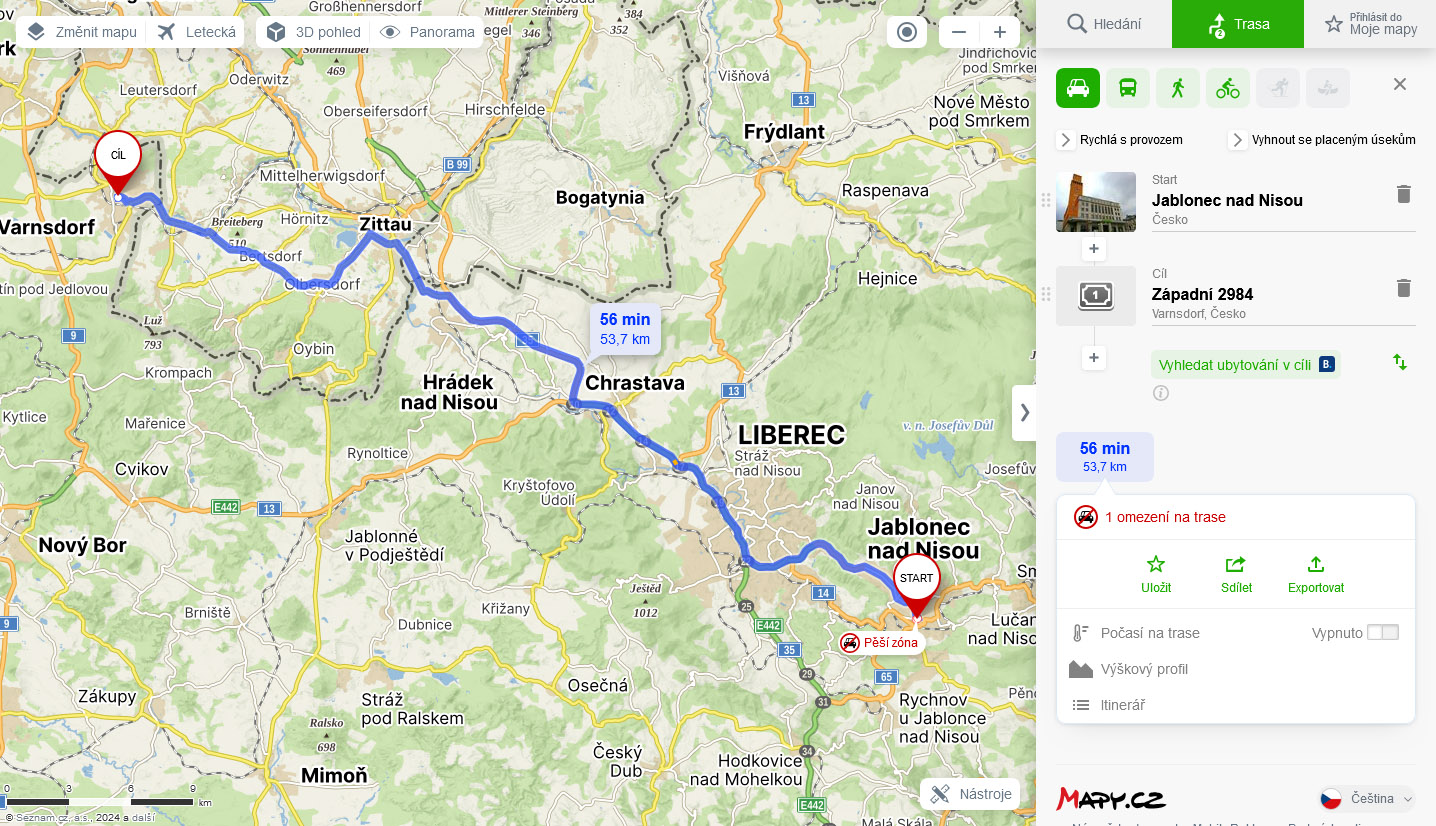
\includegraphics[width=\textwidth, keepaspectratio]{rijen_cestak_1}
	
	R3 si výši cestovného vypočítá jako počet kilometrů podle portálu \href{mapy.cz}{mapy.cz}, kde zadá cestu ze svého bydliště do místa utkání. Z Jablonce nad Nisou ke sportovní hale ve Varnsdorfu to činí 54 kilometrů. Protože jede i zpět do místa bydliště, má nárok i na proplacení této cesty. Sazba za jeden kilometr činí 4,5 Kč a tudíž má R3 nárok na $2 \cdot 54 \cdot 4,5 = 243$ Kč.
	
	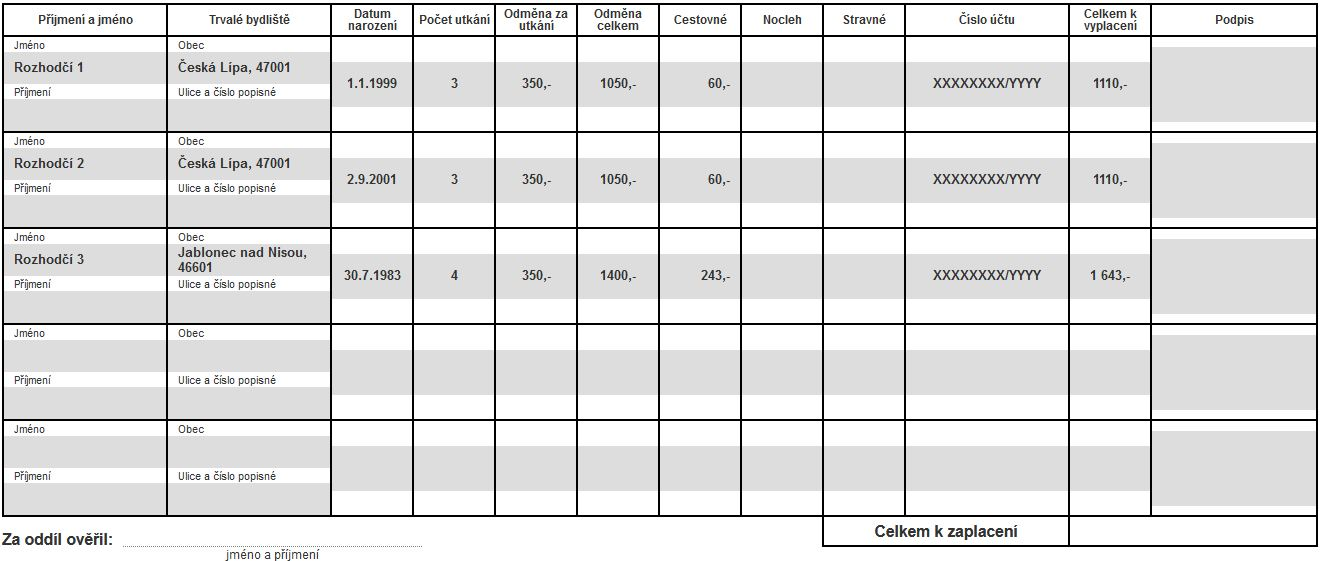
\includegraphics[width=\textwidth, keepaspectratio]{rijen-2024-vyplatnice-1}
\end{admonition-info}

\pagebreak
\clanek{Potvrzování zápisů}{a omlouvání z nominací}
KRD si dovoluje připomenout vaší povinnost potvrzovat zápisy o utkání. Ideální je potvrdit je ihned po skončení utkání, \textbf{nejpozději však do neděle 18:00 daného hracího víkendu}. KRD apeluje na rozhodčí, aby zápisy kontrolovali a potvrzovali co nejdříve to je možné. Předejdete tím možným reklamacím a chybám v zápise. Při prvním nepotvrzení obdržíte napomenutí. \textbf{Při opakovaných prohřešcích pak následuje finanční  ve výši 300 Kč za provinění}. V případě problémů se zápisem kontaktujte Blanku Procházkovou.

\begin{admonition-info}{Manažerka regionu}
	\begin{flushleft}
		\raisebox{-0.5\height}{
\includegraphics[width=2.6cm, keepaspectratio]{blanka_prochazkova}} % Replace with your logo file
		\hspace{0.5em} % Space between logo and text
		\parbox{8cm}{ % Width of the parbox can be adjusted
			\textcolor{cfblue}{{\large \GeogrotesqueCondensedBold{Blanka Procházková}}}
			\\
			{\small \href{tel:608956579}{+420 608 956 579}}\\
			{\small \href{mailto:prochazkova@ceskyflorbal.cz}{prochazkova@ceskyflorbal.cz}}
		}
	\end{flushleft}
\end{admonition-info}

Pokud se nemůžete zúčastnit nominovaného zápasu, máte povinnost se omluvit. \textbf{Na omluvu máte čas nejpozději do pondělí 23:59 před daným hracím víkendem} a je nutné kontaktovat koordinátora rozhodčích. Při pozdní omluvě se již bude nahlížet na důvod Vaší omluvy, podle kterého vám může, ale nemusí, být udělena finanční pokuta.

\begin{admonition-info}{Koordinátor rozhodčích}
    \begin{flushleft}
	\raisebox{-0.5\height}{
\includegraphics[width=2.6cm, keepaspectratio]{jakub_prochazka}} % Replace with your logo file
	\hspace{0.5em} % Space between logo and text
	\parbox{8cm}{ % Width of the parbox can be adjusted
		\textcolor{cfblue}{{\large \GeogrotesqueCondensedBold{Jakub Procházka}}}
		\\
		{\small \href{tel:731519989}{+420 731 519 989}}\\
		{\small \href{mailto:prochazka@ceskyflorbal.cz}{prochazka@ceskyflorbal.cz}}
	}
\end{flushleft}
\end{admonition-info}

\pagebreak
\clanek{Novinky}{a výhled do listopadu}
V listopadu nás čeká několik vzdělávacích seminářů, na které by chtěla KRD upozornit. Pro mladé naděje našeho regionu jsme si 4. a 5. listopadu přichystali semináře na téma \textbf{Pohyb 1 a signalizace}, které se uskuteční v Libereckém Storingu a respektive ve Sportovním areálu Most. Pro ostřílené foukače máme nachystaný seminář na téma \textbf{Vnímání utkání}, který proběhne 7.11.2024 online a 14.11. proběhne v Libereckém Storingu seminář na téma \textbf{Role rozhodčího a budování páru}. Na semináře vás může přihlásit sekretář vašeho oddílu, nebo se můžete sami přihlásit ve FISu v záložce \textbf{Osoba} $\to$ \textbf{Přihlášky ke školení}. Seznam všech vypsaných seminářů najdete v \href{https://www.ceskyflorbal.cz/calendar/?filter%5BmanagingAuthority%5D=2&filter%5BcommitteeType%5D=5}{kalendáři Českého florbalu}.

\begin{table}[h]
	\centering
	\renewcommand{\arraystretch}{2}
	\begin{tabular}{| r | l | l | l |}
	\hline
	04. 11. 2024 & Pohyb I + signalizace & Licence E & Liberec storing \\
	\hline
	05. 11. 2024 & Pohyb I + signalizace & Licence E & Sportovní Areály Most \\
	\hline
	07. 11. 2024 & Vnímání utkání & Licence C & online teams ÚsaLb \\
	\hline
	14. 11. 2024 & Role rozhodčího + budování páru I & Licence D & Storing Liberec \\
	\hline
	27. 11. 2024 & Emoce I + tresty I & Licence E & Liberec storing	\\
	\hline
	\end{tabular}
\end{table}

Od listopadu také spouštíme jednu novinku, a to je \textbf{měsíční Kahoot!} Každý měsíc budeme soutěžit a ti, co se umístí na prvních příčkách, se mohou těšit na zajímavé ceny.

\end{document}